% Options for packages loaded elsewhere
% Options for packages loaded elsewhere
\PassOptionsToPackage{unicode}{hyperref}
\PassOptionsToPackage{hyphens}{url}
%
\documentclass[
  ignorenonframetext,
  aspectratio=169,
  russian,
]{beamer}
\newif\ifbibliography
\usepackage{pgfpages}
\setbeamertemplate{caption}[numbered]
\setbeamertemplate{caption label separator}{: }
\setbeamercolor{caption name}{fg=normal text.fg}
\beamertemplatenavigationsymbolshorizontal
% Prevent slide breaks in the middle of a paragraph
\widowpenalties 1 10000
\raggedbottom
\AtBeginPart{
  \frame{\partpage}
}
\AtBeginSection{
  \ifbibliography
  \else
    \frame{\sectionpage}
  \fi
}
\AtBeginSubsection{
  \frame{\subsectionpage}
}
\usepackage{iftex}
\ifPDFTeX
  \usepackage[T1]{fontenc}
  \usepackage[utf8]{inputenc}
  \usepackage{textcomp} % provide euro and other symbols
\else % if luatex or xetex
  \usepackage{unicode-math} % this also loads fontspec
  \defaultfontfeatures{Scale=MatchLowercase}
  \defaultfontfeatures[\rmfamily]{Ligatures=TeX,Scale=1}
\fi
\usepackage{lmodern}

\usefonttheme{serif} % use mainfont rather than sansfont for slide text
\ifPDFTeX\else
  % xetex/luatex font selection
  \setmainfont[]{DejaVu Serif}
  \setsansfont[]{DejaVu Sans}
  \setmonofont[]{DejaVu Sans Mono}
\fi
% Use upquote if available, for straight quotes in verbatim environments
\IfFileExists{upquote.sty}{\usepackage{upquote}}{}
\IfFileExists{microtype.sty}{% use microtype if available
  \usepackage[]{microtype}
  \UseMicrotypeSet[protrusion]{basicmath} % disable protrusion for tt fonts
}{}


\usepackage{longtable,booktabs,array}
\usepackage{calc} % for calculating minipage widths
\usepackage{caption}
% Make caption package work with longtable
\makeatletter
\def\fnum@table{\tablename~\thetable}
\makeatother
\usepackage{graphicx}
\makeatletter
\newsavebox\pandoc@box
\newcommand*\pandocbounded[1]{% scales image to fit in text height/width
  \sbox\pandoc@box{#1}%
  \Gscale@div\@tempa{\textheight}{\dimexpr\ht\pandoc@box+\dp\pandoc@box\relax}%
  \Gscale@div\@tempb{\linewidth}{\wd\pandoc@box}%
  \ifdim\@tempb\p@<\@tempa\p@\let\@tempa\@tempb\fi% select the smaller of both
  \ifdim\@tempa\p@<\p@\scalebox{\@tempa}{\usebox\pandoc@box}%
  \else\usebox{\pandoc@box}%
  \fi%
}
% Set default figure placement to htbp
\def\fps@figure{htbp}
\makeatother



\ifLuaTeX
\usepackage[bidi=basic,provide=*]{babel}
\else
\usepackage[bidi=default,provide=*]{babel}
\fi
\ifPDFTeX
\else
\babelfont{rm}[]{DejaVu Serif}
\fi
% get rid of language-specific shorthands (see #6817):
\let\LanguageShortHands\languageshorthands
\def\languageshorthands#1{}


\setlength{\emergencystretch}{3em} % prevent overfull lines

\providecommand{\tightlist}{%
  \setlength{\itemsep}{0pt}\setlength{\parskip}{0pt}}



 

\usepackage[]{csquotes}

\IfFileExists{plex-otf.sty}{
  %% Full TeXlive
  % \usepackage[%
  %   % math,
  %   RM={Scale=0.94},SS={Scale=0.94},SScon={Scale=0.94},TT={Scale=MatchLowercase,FakeStretch=0.9},DefaultFeatures={Ligatures=Common}
  % ]{plex-otf}
}{
  %% Local fallback fonts with Cyrillic support
  \usepackage{fontspec}
  \usefonttheme{professionalfonts}
  \AtBeginDocument{%
    \setmainfont{DejaVu Serif}
    \setsansfont{DejaVu Sans}
    \setmonofont{DejaVu Sans Mono}%
  }
}

%%% Load theme
% https://deic.uab.cat/~iblanes/beamer_gallery/
\IfFileExists{beamerthemegotham.sty}{
  %% Full TeXlive
  \usetheme{gotham}
  \gothamset{
    numbering=totalpagenumber,
    parttocframe default=off,
    sectiontocframe default=off,
    subsectiontocframe default=off,
  }
}{
  %% TinyTeX
  \usetheme{Madrid}
}
\makeatletter
\@ifpackageloaded{caption}{}{\usepackage{caption}}
\AtBeginDocument{%
\ifdefined\contentsname
  \renewcommand*\contentsname{Содержание}
\else
  \newcommand\contentsname{Содержание}
\fi
\ifdefined\listfigurename
  \renewcommand*\listfigurename{Список иллюстраций}
\else
  \newcommand\listfigurename{Список иллюстраций}
\fi
\ifdefined\listtablename
  \renewcommand*\listtablename{Список таблиц}
\else
  \newcommand\listtablename{Список таблиц}
\fi
\ifdefined\figurename
  \renewcommand*\figurename{Рисунок}
\else
  \newcommand\figurename{Рисунок}
\fi
\ifdefined\tablename
  \renewcommand*\tablename{Таблица}
\else
  \newcommand\tablename{Таблица}
\fi
}
\@ifpackageloaded{float}{}{\usepackage{float}}
\floatstyle{ruled}
\@ifundefined{c@chapter}{\newfloat{codelisting}{h}{lop}}{\newfloat{codelisting}{h}{lop}[chapter]}
\floatname{codelisting}{Список}
\newcommand*\listoflistings{\listof{codelisting}{Листинги}}
\makeatother
\makeatletter
\makeatother
\makeatletter
\@ifpackageloaded{caption}{}{\usepackage{caption}}
\@ifpackageloaded{subcaption}{}{\usepackage{subcaption}}
\makeatother

\usepackage{bookmark}
\IfFileExists{xurl.sty}{\usepackage{xurl}}{} % add URL line breaks if available
\urlstyle{same}
\hypersetup{
  pdftitle={Внешний курс №1},
  pdfauthor={Трусова Алина Александровна},
  pdflang={ru-RU},
  hidelinks,
  pdfcreator={LaTeX via pandoc}}


\title{Внешний курс №1}
\subtitle{Безопасность в сети}
\author{Трусова Алина Александровна}
\date{}

\begin{document}
\frame{\titlepage}

\renewcommand*\contentsname{Содержание}
\begin{frame}[allowframebreaks]
  \frametitle{Содержание}
  \setcounter{tocdepth}{2}
  \tableofcontents
\end{frame}
\setcounter{tocdepth}{2}
\tableofcontents
}

\section{1. Цель
работы}\label{ux446ux435ux43bux44c-ux440ux430ux431ux43eux442ux44b}

\begin{frame}{1. Цель работы}
Выполнение контрольных заданий первого блока внешнего курса
\enquote{Основы Кибербезопасности}
\end{frame}

\section{\texorpdfstring{2. Выполнение заданий блока \enquote{Основы
Кибербезопасности}}{2. Выполнение заданий блока ``Основы Кибербезопасности''}}\label{ux432ux44bux43fux43eux43bux43dux435ux43dux438ux435-ux437ux430ux434ux430ux43dux438ux439-ux431ux43bux43eux43aux430-ux43eux441ux43dux43eux432ux44b-ux43aux438ux431ux435ux440ux431ux435ux437ux43eux43fux430ux441ux43dux43eux441ux442ux438}

\begin{frame}{2.1 Как работает интернет: базовые сетевые протоколы}
\phantomsection\label{ux43aux430ux43a-ux440ux430ux431ux43eux442ux430ux435ux442-ux438ux43dux442ux435ux440ux43dux435ux442-ux431ux430ux437ux43eux432ux44bux435-ux441ux435ux442ux435ux432ux44bux435-ux43fux440ux43eux442ux43eux43aux43eux43bux44b}
\end{frame}

\begin{frame}
UDP - протокол сетевого уровня TCP - протокол транспортного уровня HTTPS
- протокол прикладного уровня IP - протокол сетевого уровня, поэтому
ответ HTTPS (рис. {[}-@fig:001{]}).

\begin{figure}

{\centering 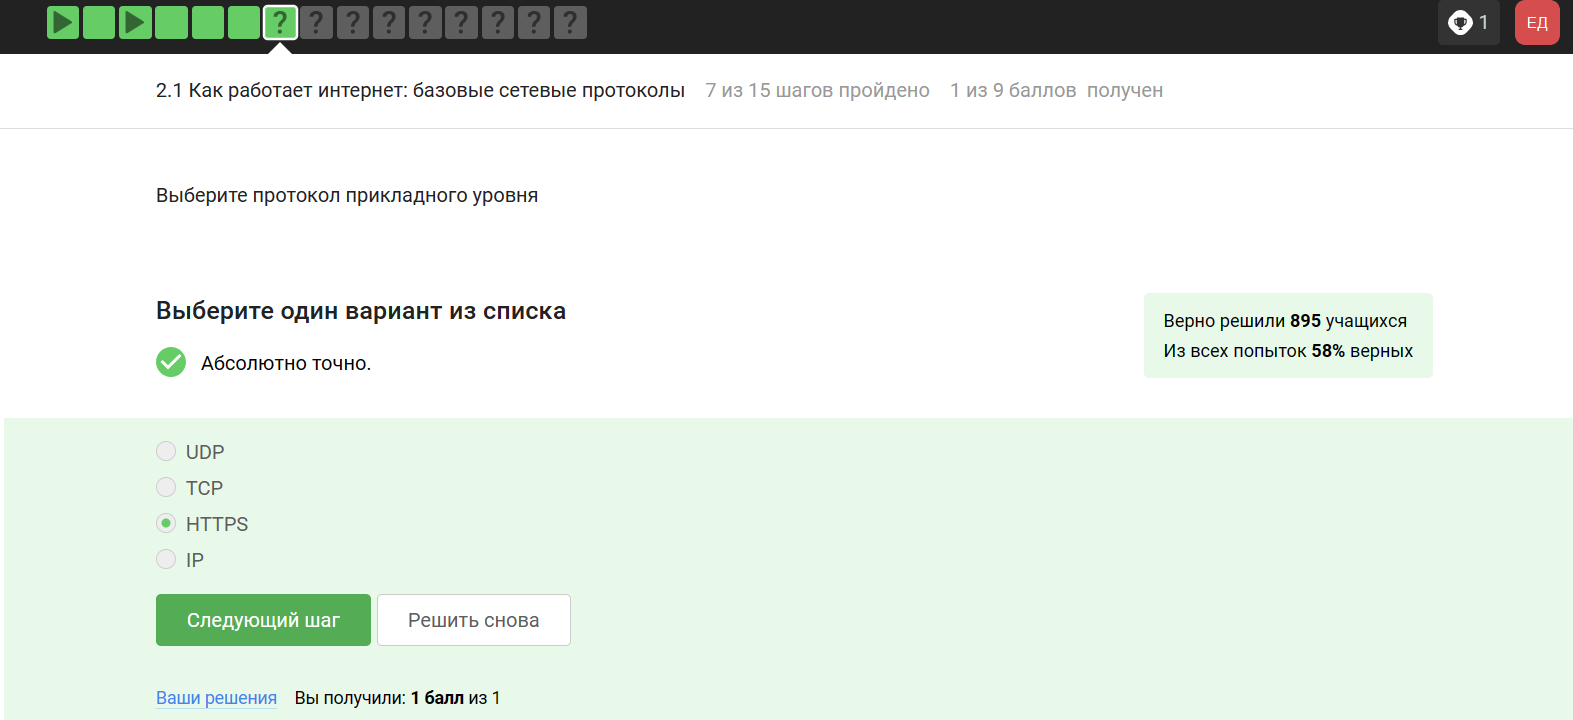
\includegraphics[width=0.7\linewidth,height=\textheight,keepaspectratio]{../report/image/1.PNG}

}

\caption{Вопрос 2.1.1}

\end{figure}%
\end{frame}

\begin{frame}
Ранее было упомянуто, что протокол TCP - transmission control protocol -
работает на транспортном уровне (рис. {[}-@fig:002{]}).

\begin{figure}

{\centering 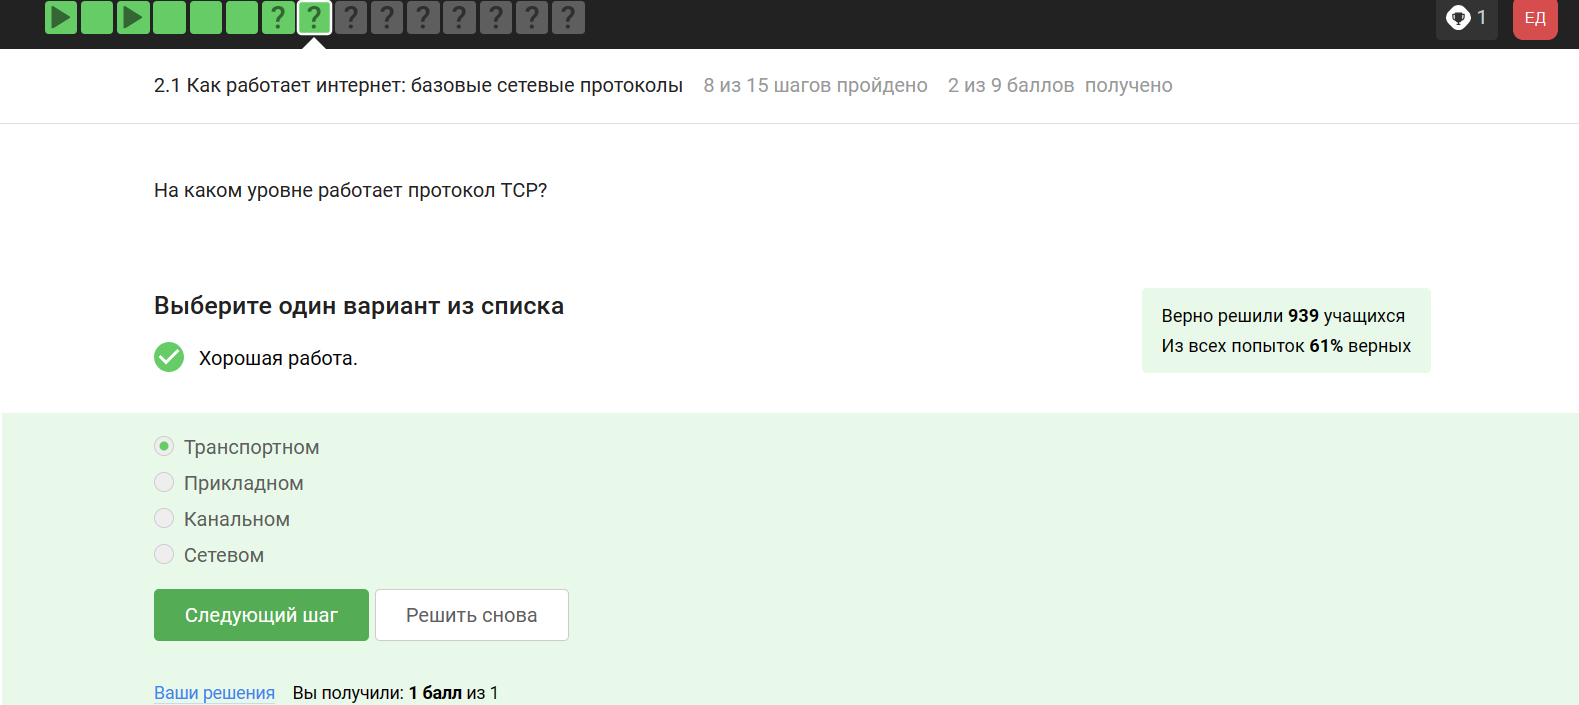
\includegraphics[width=0.7\linewidth,height=\textheight,keepaspectratio]{../report/image/2.PNG}

}

\caption{Вопрос 2.1.2}

\end{figure}%
\end{frame}

\begin{frame}
В адресе типа IPv4 не может быть чисел больше 255, поэтому первые два
варианта не подходят (рис. {[}-@fig:003{]}).

\begin{figure}

{\centering 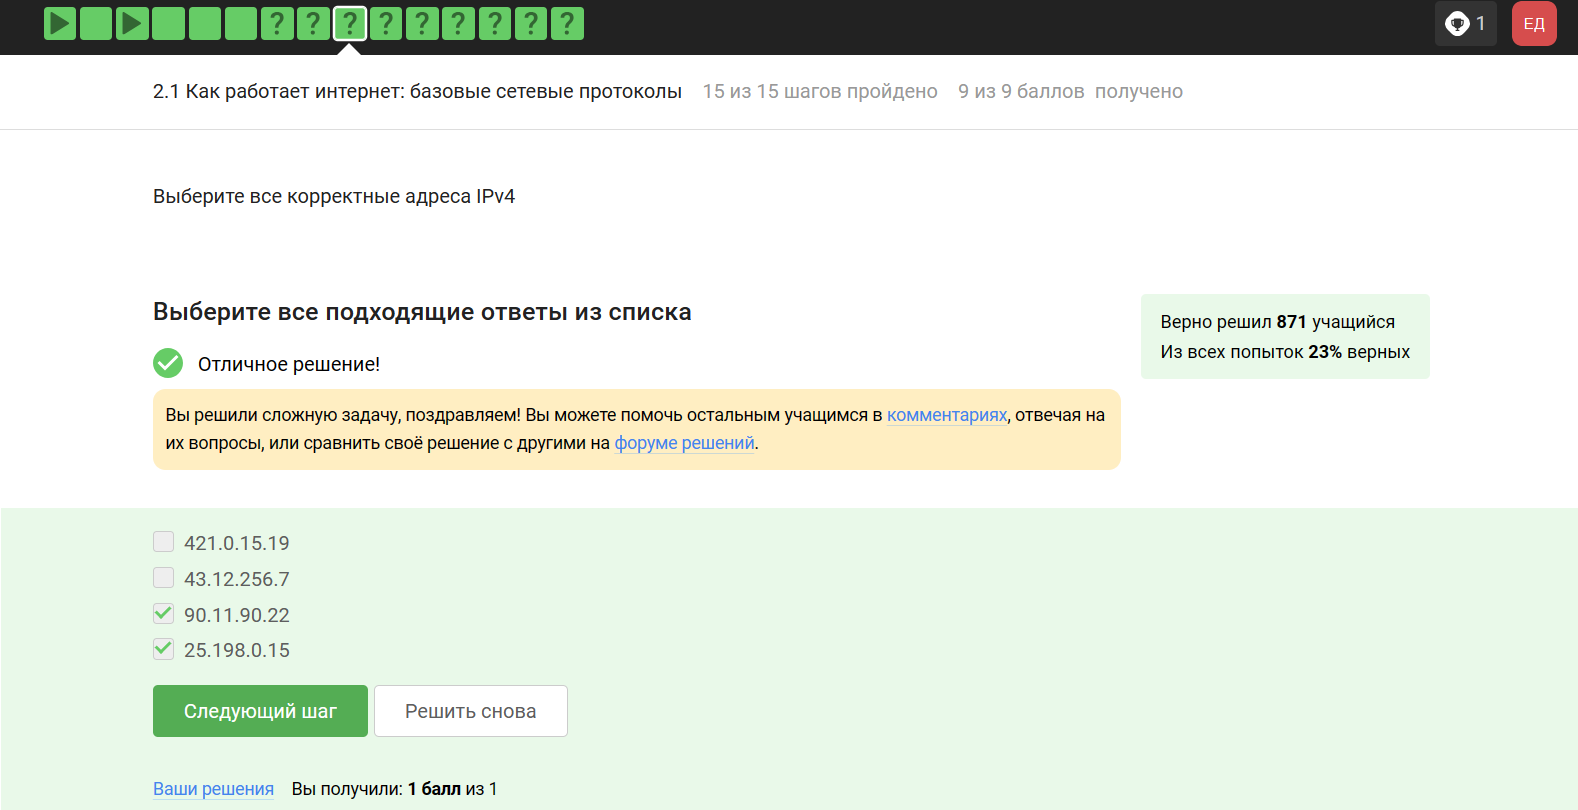
\includegraphics[width=0.7\linewidth,height=\textheight,keepaspectratio]{../report/image/3.PNG}

}

\caption{Вопрос 2.1.3}

\end{figure}%
\end{frame}

\begin{frame}
DNS-сервер, Domain name server --- приложение, предназначенное для
ответов на DNS-запросы по соответствующему протоколу Обязательное
условие -- Сопоставление сервером доменных имен доменного имени с
IP-адресом называется разрешением имени и адреса (рис. {[}-@fig:004{]}).

\begin{figure}

{\centering 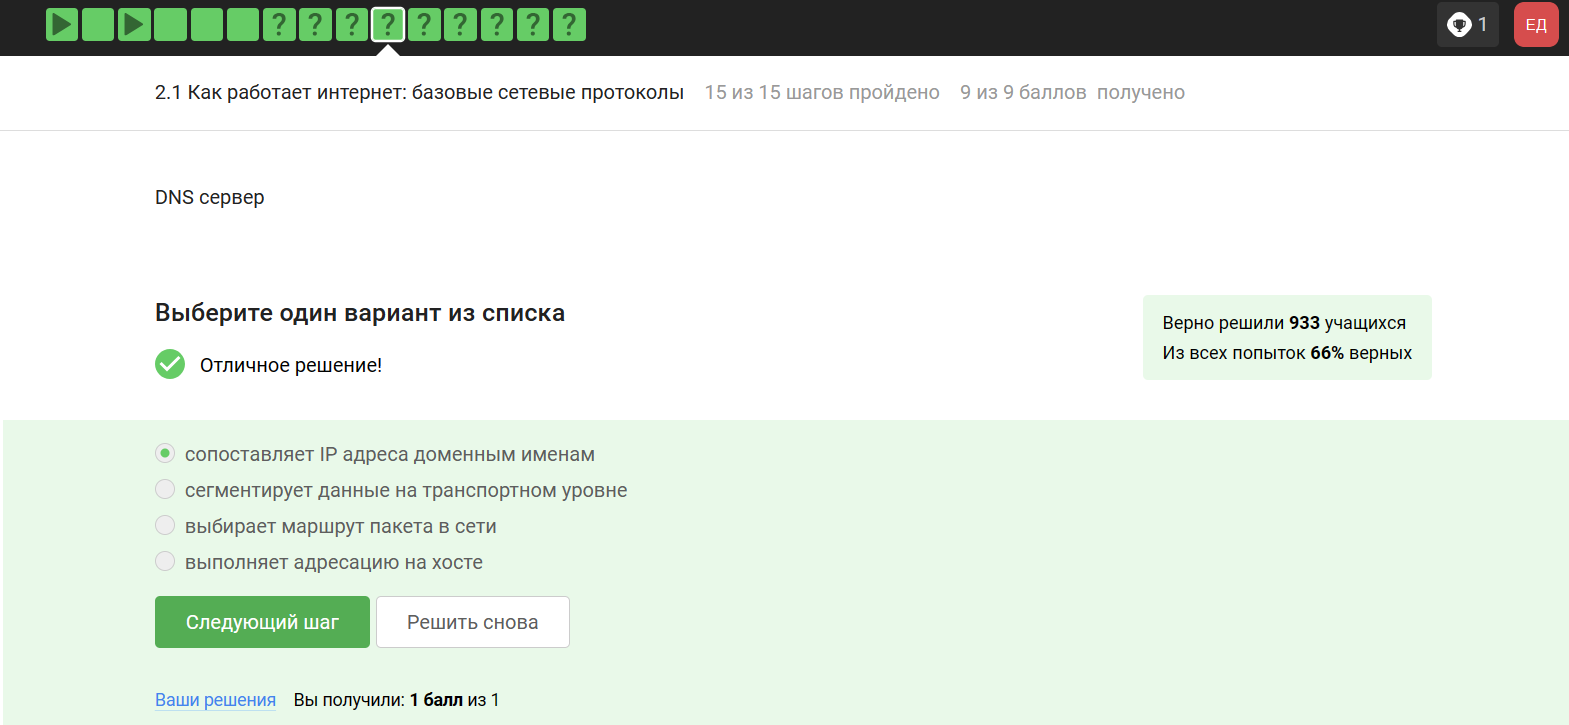
\includegraphics[width=0.7\linewidth,height=\textheight,keepaspectratio]{../report/image/4.PNG}

}

\caption{Вопрос 2.1.4}

\end{figure}%

Распределение протоколов в модели TCP/IP:

\begin{itemize}[<+->]
\item
  Прикладной уровень (Application Layer): HTTP, RTSP, FTP, DNS.
\item
  Транспортный уровень (Transport Layer): TCP, UDP, SCTP, DCCP.
\item
  Сетевой (Межсетевой) уровень (Network Layer): IP.
\end{itemize}
\end{frame}

\begin{frame}
\begin{itemize}[<+->]
\tightlist
\item
  Уровень сетевого доступа (Канальный) (Link Layer): Ethernet, IEEE
  802.11, WLAN, SLIP, Token Ring, ATM и MPLS. (рис. {[}-@fig:005{]}).
\end{itemize}

\begin{figure}

{\centering 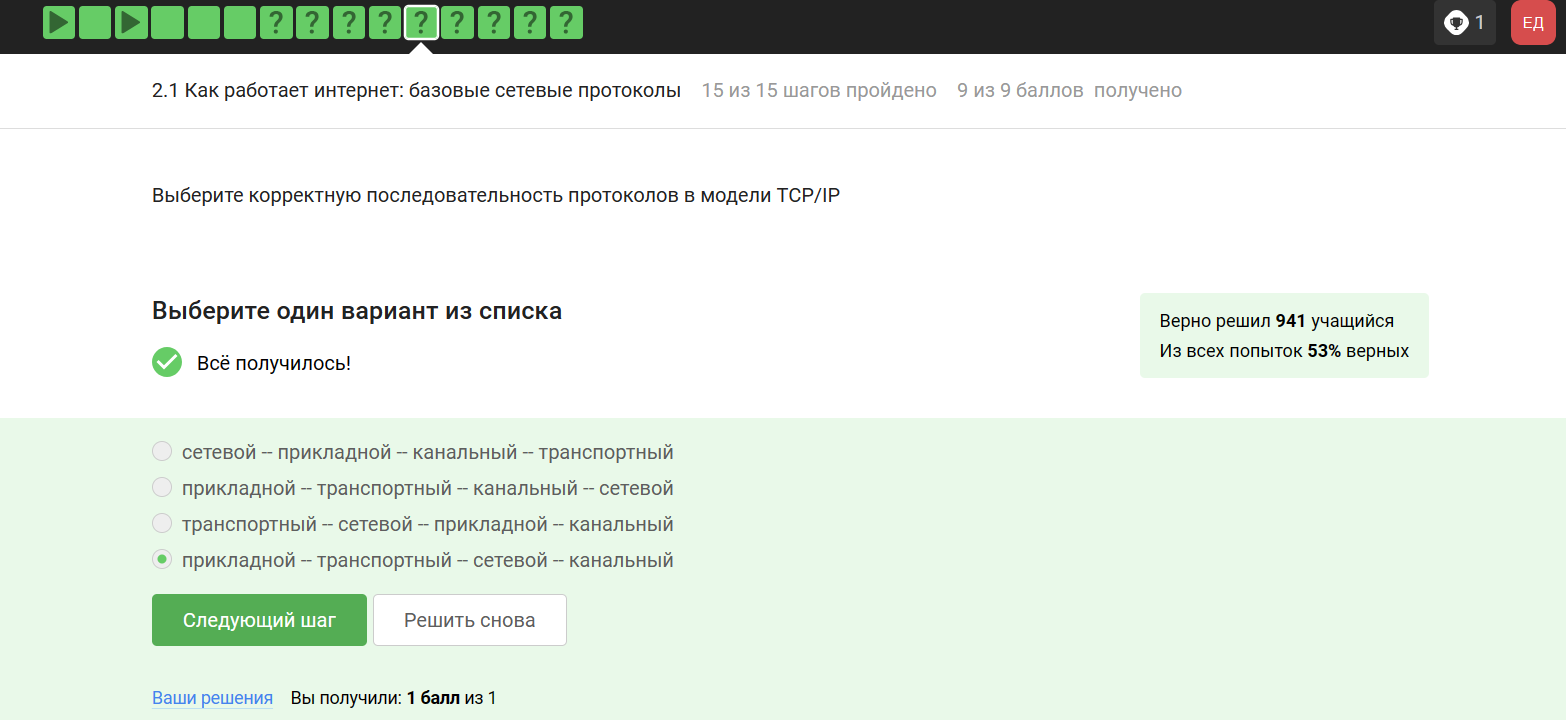
\includegraphics[width=0.7\linewidth,height=\textheight,keepaspectratio]{../report/image/5.PNG}

}

\caption{Вопрос 2.1.5}

\end{figure}%
\end{frame}

\begin{frame}
Протокол http передает не зашифрованные данные, а протокол https уже
будет передавать зашифрованные данные (рис. {[}-@fig:006{]}).

\begin{figure}

{\centering 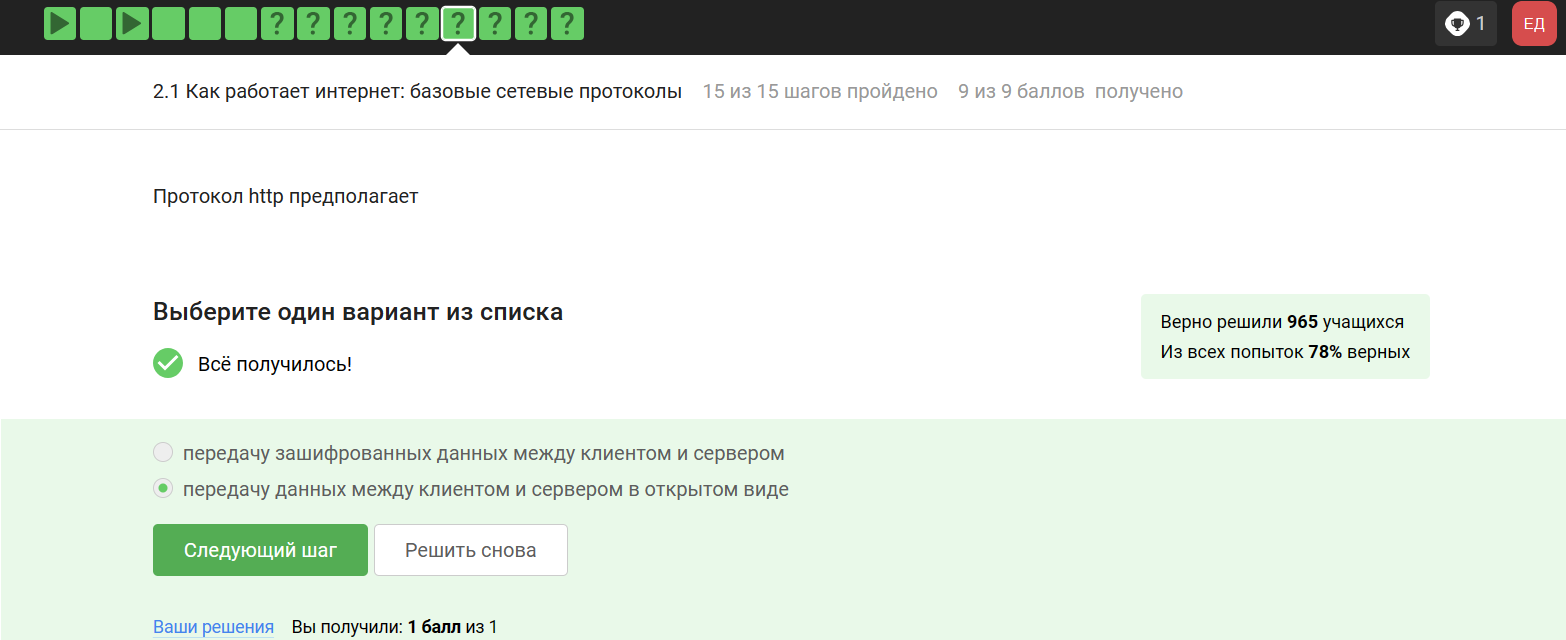
\includegraphics[width=0.7\linewidth,height=\textheight,keepaspectratio]{../report/image/6.PNG}

}

\caption{Вопрос 2.1.6}

\end{figure}%
\end{frame}

\begin{frame}
https передает зашифрованные данные, одна из фаз - передача данных,
другая должна быть рукопожатием (рис. {[}-@fig:007{]}).

\begin{figure}

{\centering 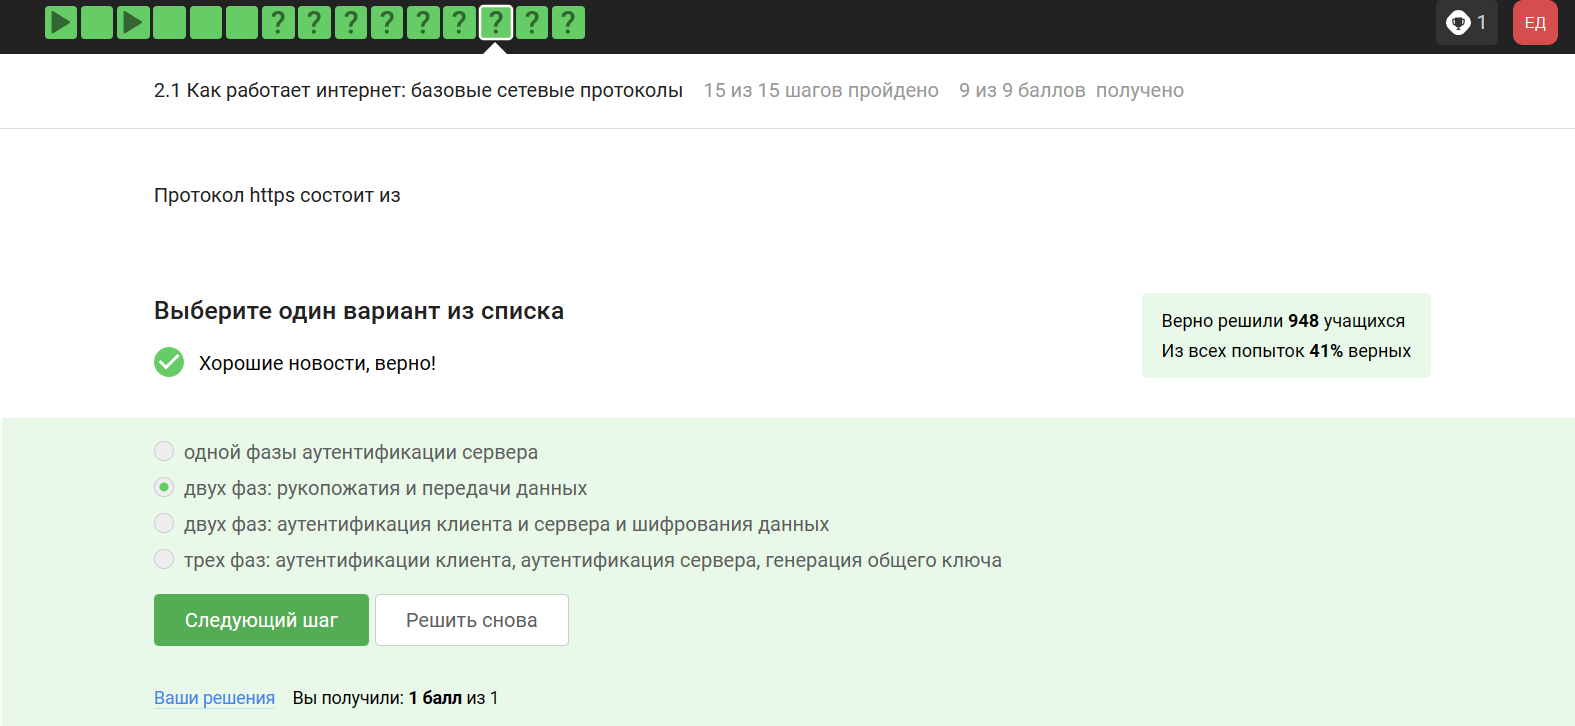
\includegraphics[width=0.7\linewidth,height=\textheight,keepaspectratio]{../report/image/7.PNG}

}

\caption{Вопрос 2.1.7}

\end{figure}%
\end{frame}

\begin{frame}
TLS определяется и клиентом, и сервером, чтобы было возможно
подключиться (рис. {[}-@fig:008{]}).

\begin{figure}

{\centering 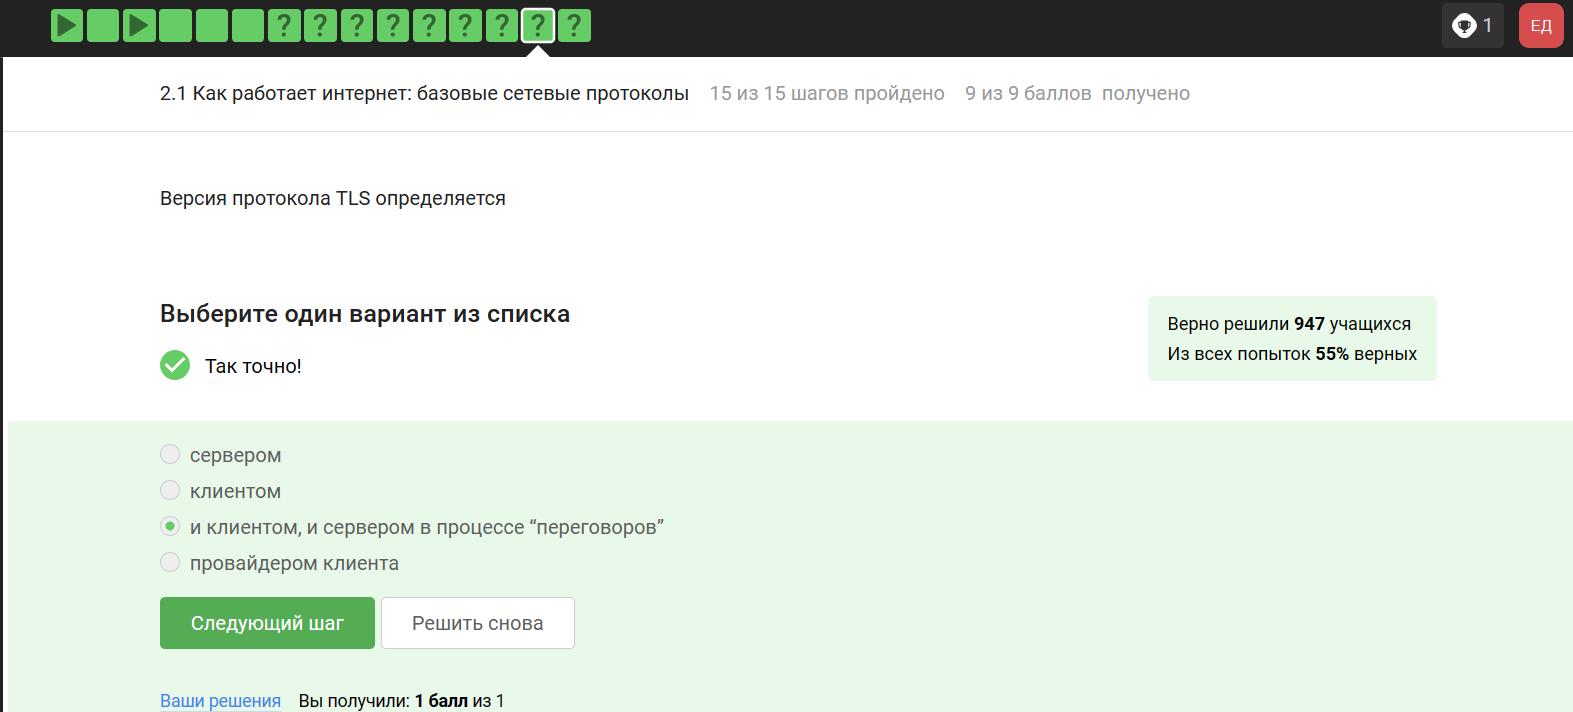
\includegraphics[width=0.7\linewidth,height=\textheight,keepaspectratio]{../report/image/8.PNG}

}

\caption{Вопрос 2.1.8}

\end{figure}%
\end{frame}

\begin{frame}
Ответ на изображении, остальные варианты в протоколе предусмотрены (рис.
{[}-@fig:009{]}).

\begin{figure}

{\centering 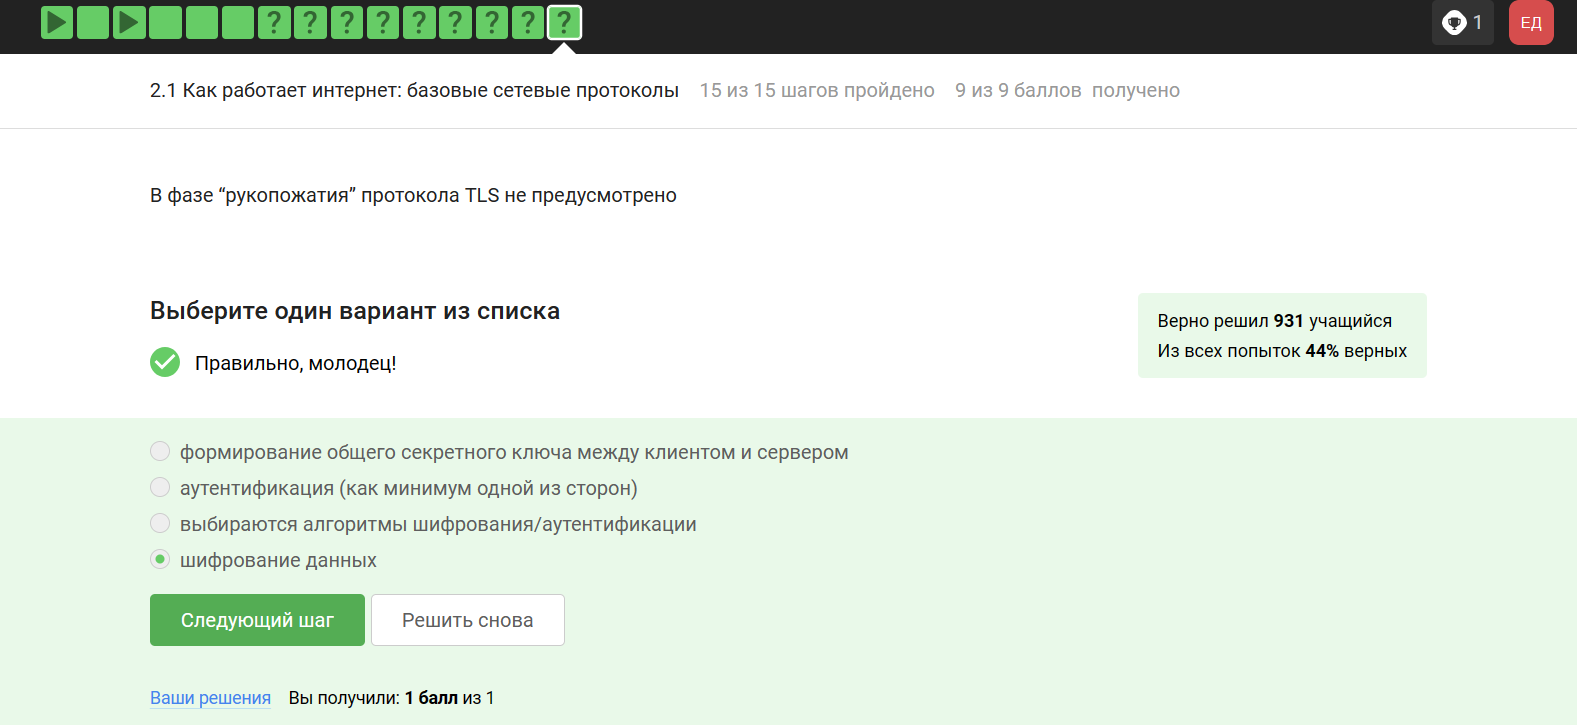
\includegraphics[width=0.7\linewidth,height=\textheight,keepaspectratio]{../report/image/9.PNG}

}

\caption{Вопрос 2.1.9}

\end{figure}%
\end{frame}

\begin{frame}{2.2 Персонализация сети}
\phantomsection\label{ux43fux435ux440ux441ux43eux43dux430ux43bux438ux437ux430ux446ux438ux44f-ux441ux435ux442ux438}
\end{frame}

\begin{frame}
Куки точно не хранят пароли и IP-адреса, а id ceccии и идентификатор
хранят (рис. {[}-@fig:010{]}).

\begin{figure}

{\centering 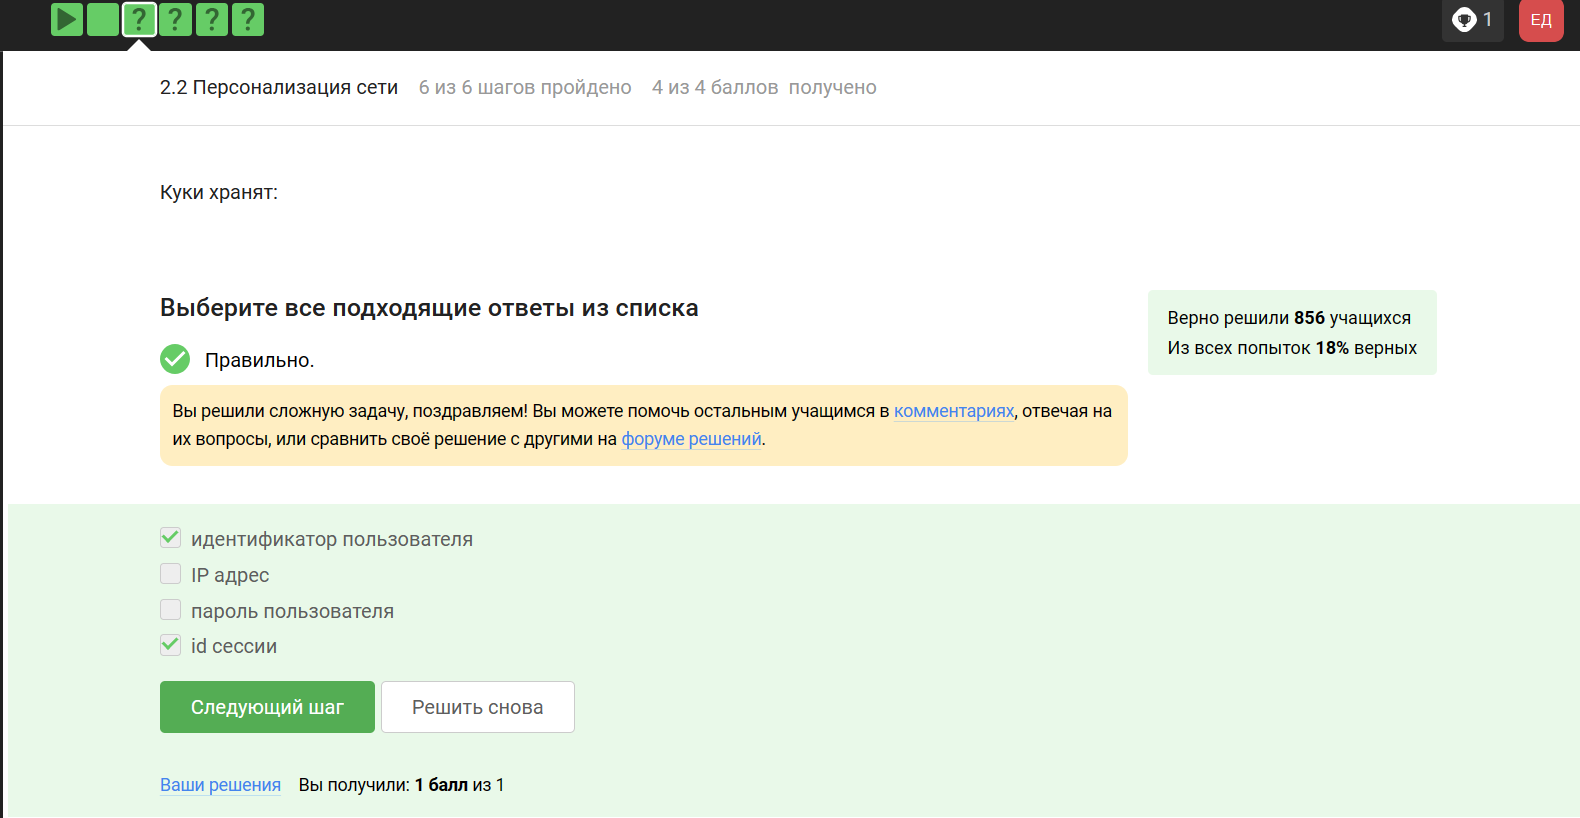
\includegraphics[width=0.7\linewidth,height=\textheight,keepaspectratio]{../report/image/10.PNG}

}

\caption{Вопрос 2.2.1}

\end{figure}%
\end{frame}

\begin{frame}
Конечно же, куки не делают соединение более надежным (рис.
{[}-@fig:011{]}).

\begin{figure}

{\centering 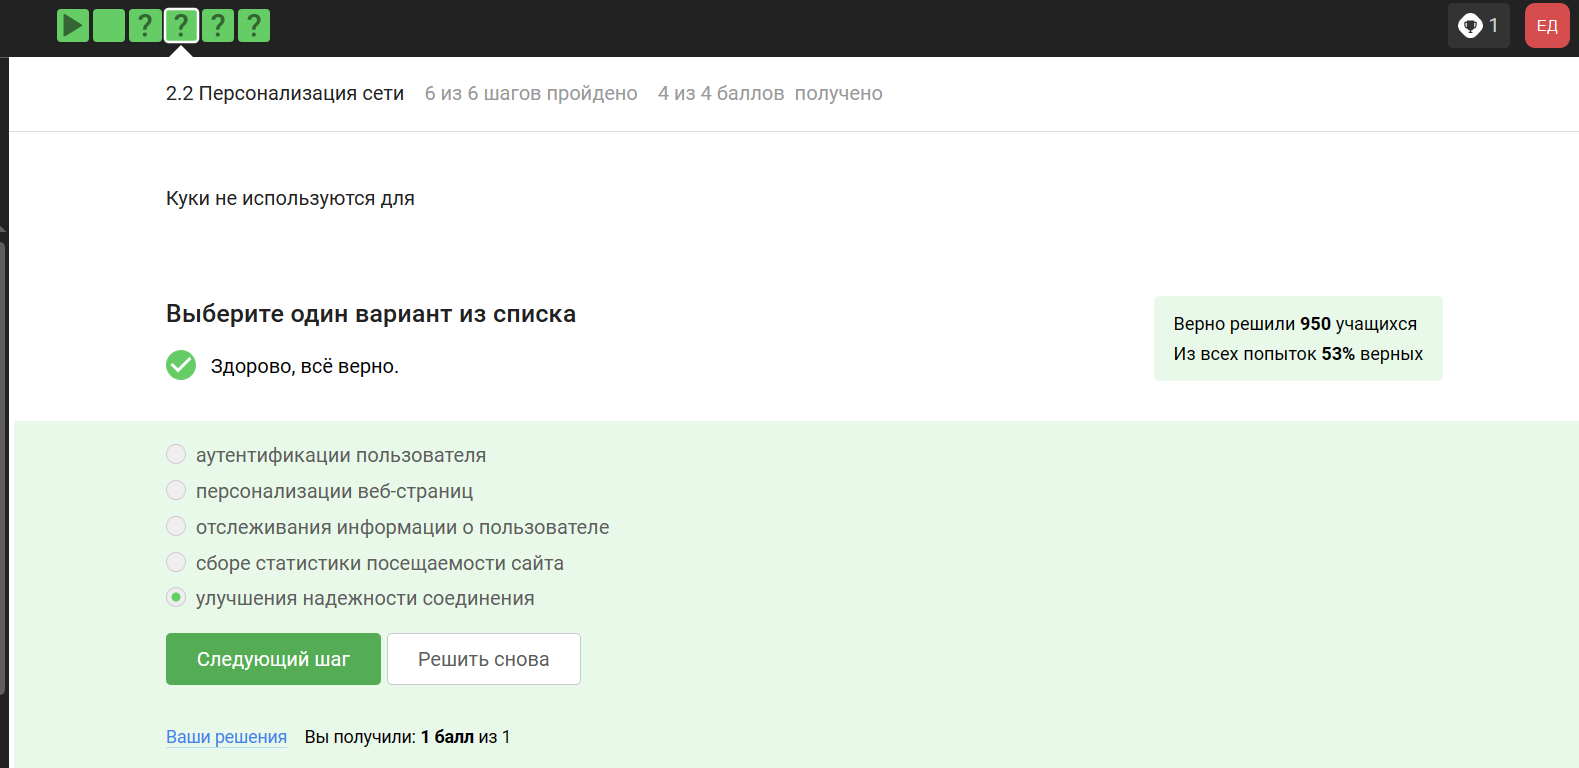
\includegraphics[width=0.7\linewidth,height=\textheight,keepaspectratio]{../report/image/11.PNG}

}

\caption{Вопрос 2.2.2}

\end{figure}%
\end{frame}

\begin{frame}
Ответ на изображении (рис. {[}-@fig:012{]}).

\begin{figure}

{\centering 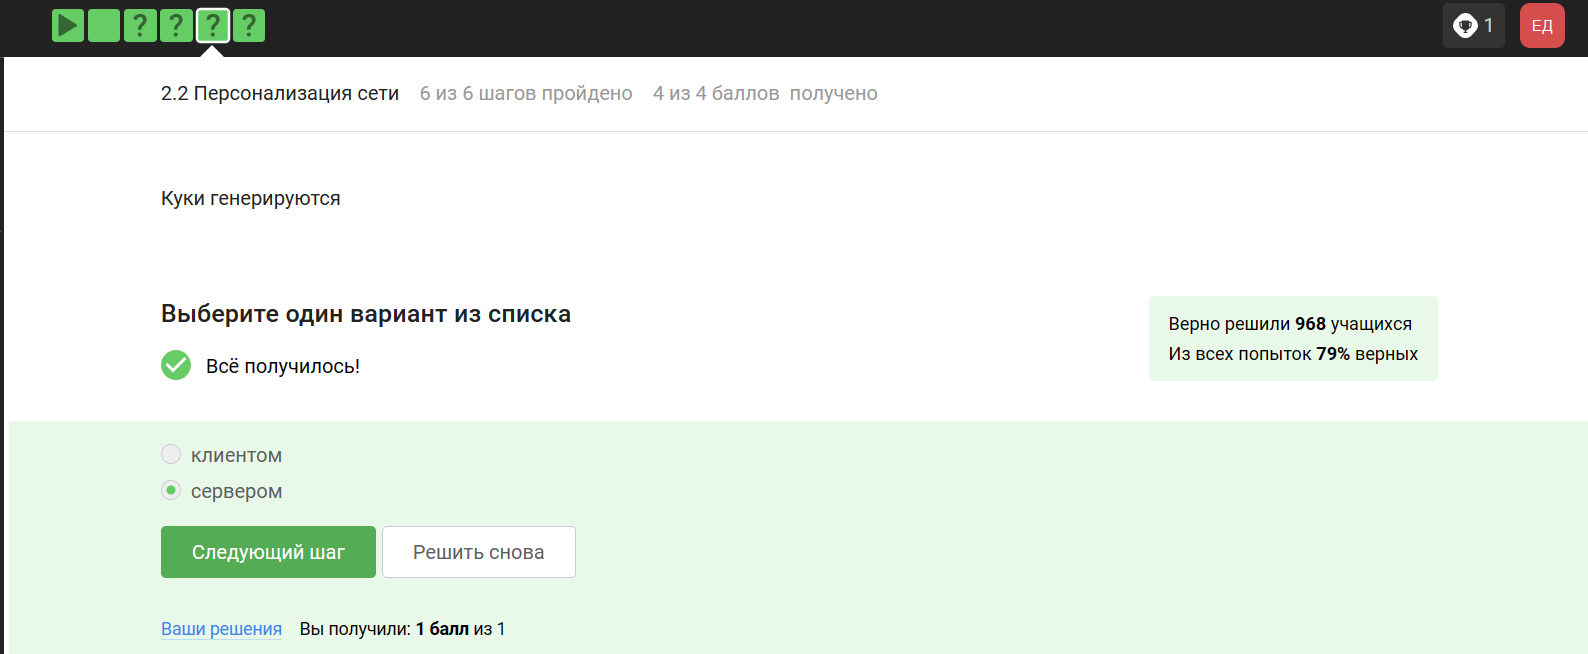
\includegraphics[width=0.7\linewidth,height=\textheight,keepaspectratio]{../report/image/12.PNG}

}

\caption{Вопрос 2.2.3}

\end{figure}%
\end{frame}

\begin{frame}
Сессионные куки хранятся в течение сессии, то есть пока используется
веб-сайт (рис. {[}-@fig:013{]}).

\begin{figure}

{\centering 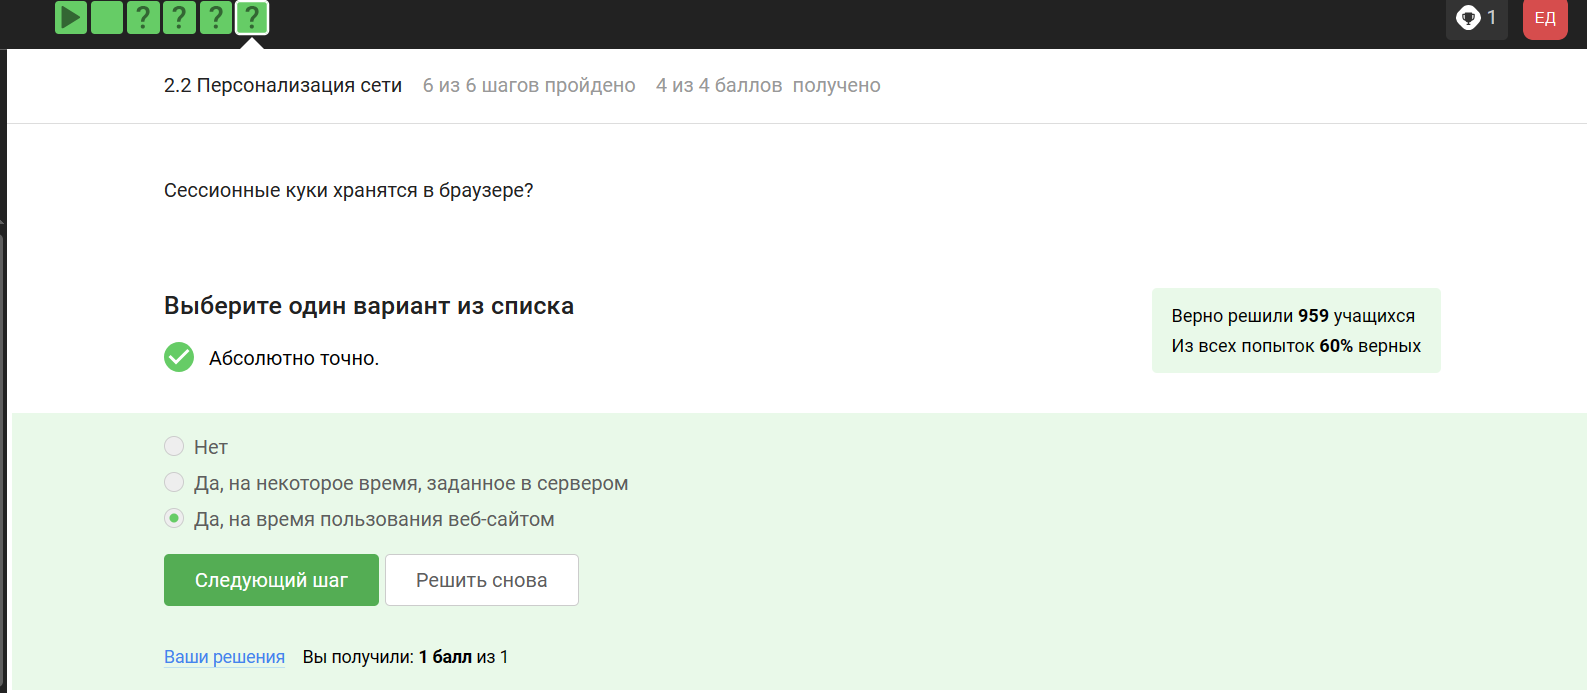
\includegraphics[width=0.7\linewidth,height=\textheight,keepaspectratio]{../report/image/13.PNG}

}

\caption{Вопрос 2.2.4}

\end{figure}%
\end{frame}

\begin{frame}{2.3 Браузер TOR. Анонимизация}
\phantomsection\label{ux431ux440ux430ux443ux437ux435ux440-tor.-ux430ux43dux43eux43dux438ux43cux438ux437ux430ux446ux438ux44f}
\end{frame}

\begin{frame}
Необходимо три узла - входной, промежуточный и выходной (рис.
{[}-@fig:014{]}).

\begin{figure}

{\centering 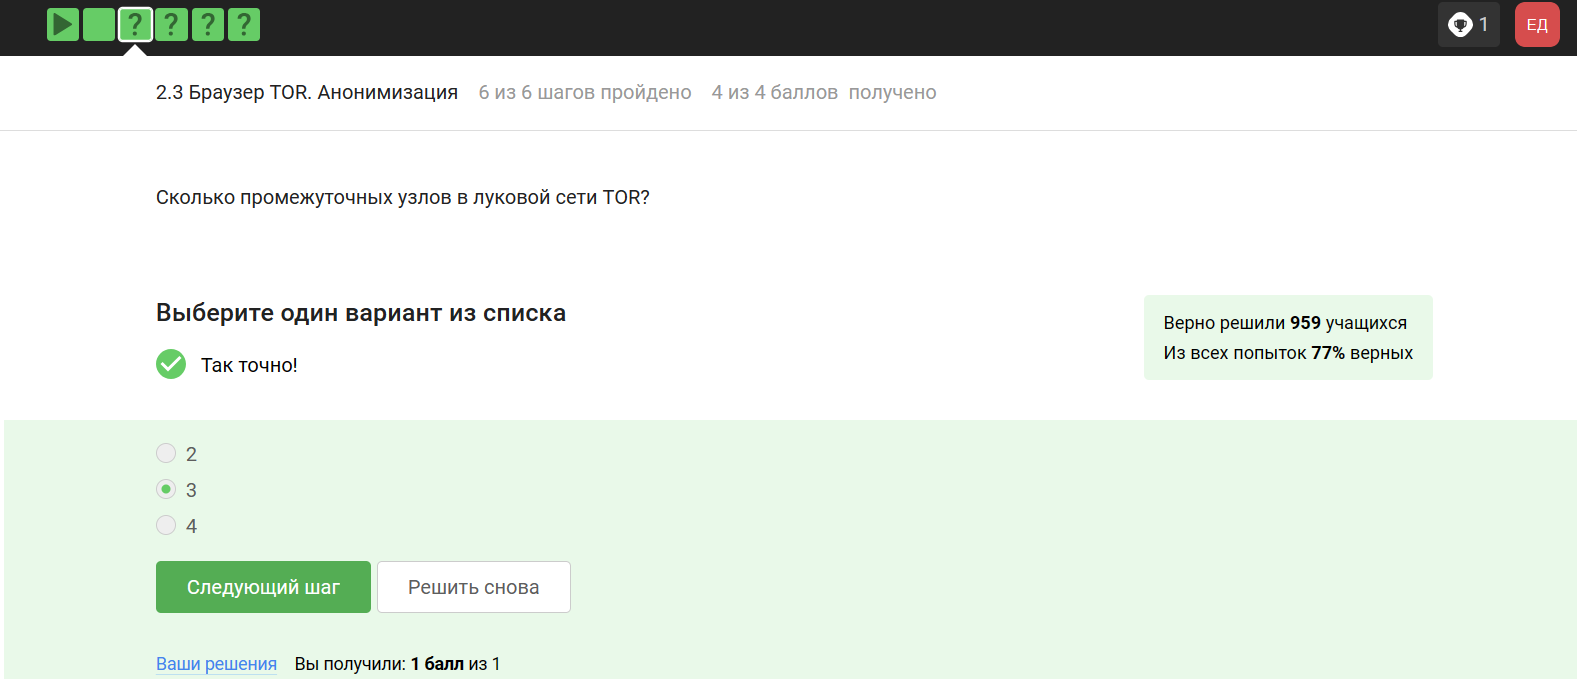
\includegraphics[width=0.7\linewidth,height=\textheight,keepaspectratio]{../report/image/14.PNG}

}

\caption{Вопрос 2.3.1}

\end{figure}%
\end{frame}

\begin{frame}
IP-адрес не должен быть известен охранному и промежуточному узлам (рис.
{[}-@fig:015{]}).

\begin{figure}

{\centering 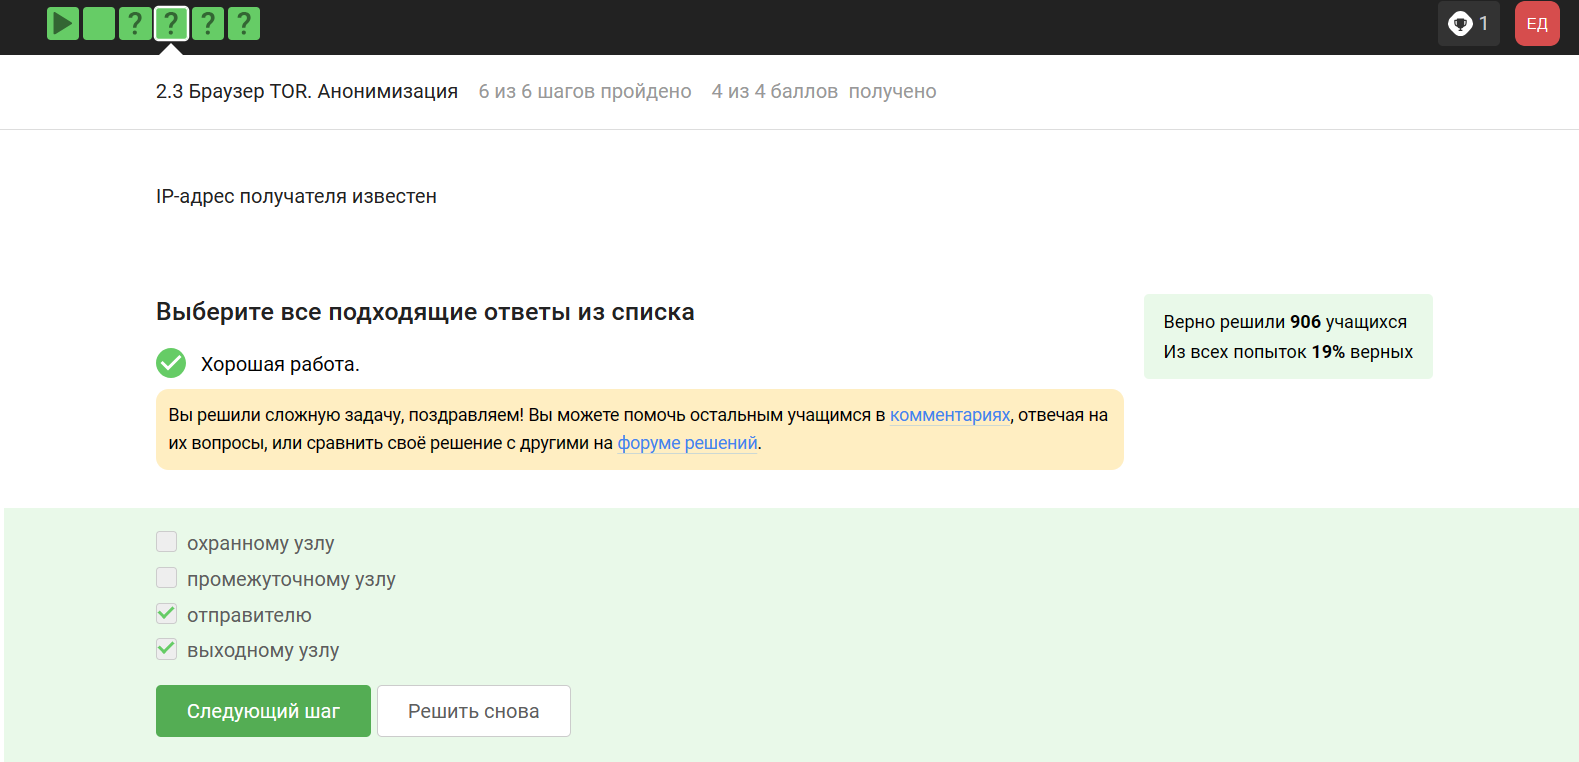
\includegraphics[width=0.7\linewidth,height=\textheight,keepaspectratio]{../report/image/15.PNG}

}

\caption{Вопрос 2.3.2}

\end{figure}%
\end{frame}

\begin{frame}
Отправитель генерирует общий секретный ключ со узлами, через которые
идет передача, то есть со всеми (рис. {[}-@fig:016{]}).

\begin{figure}

{\centering 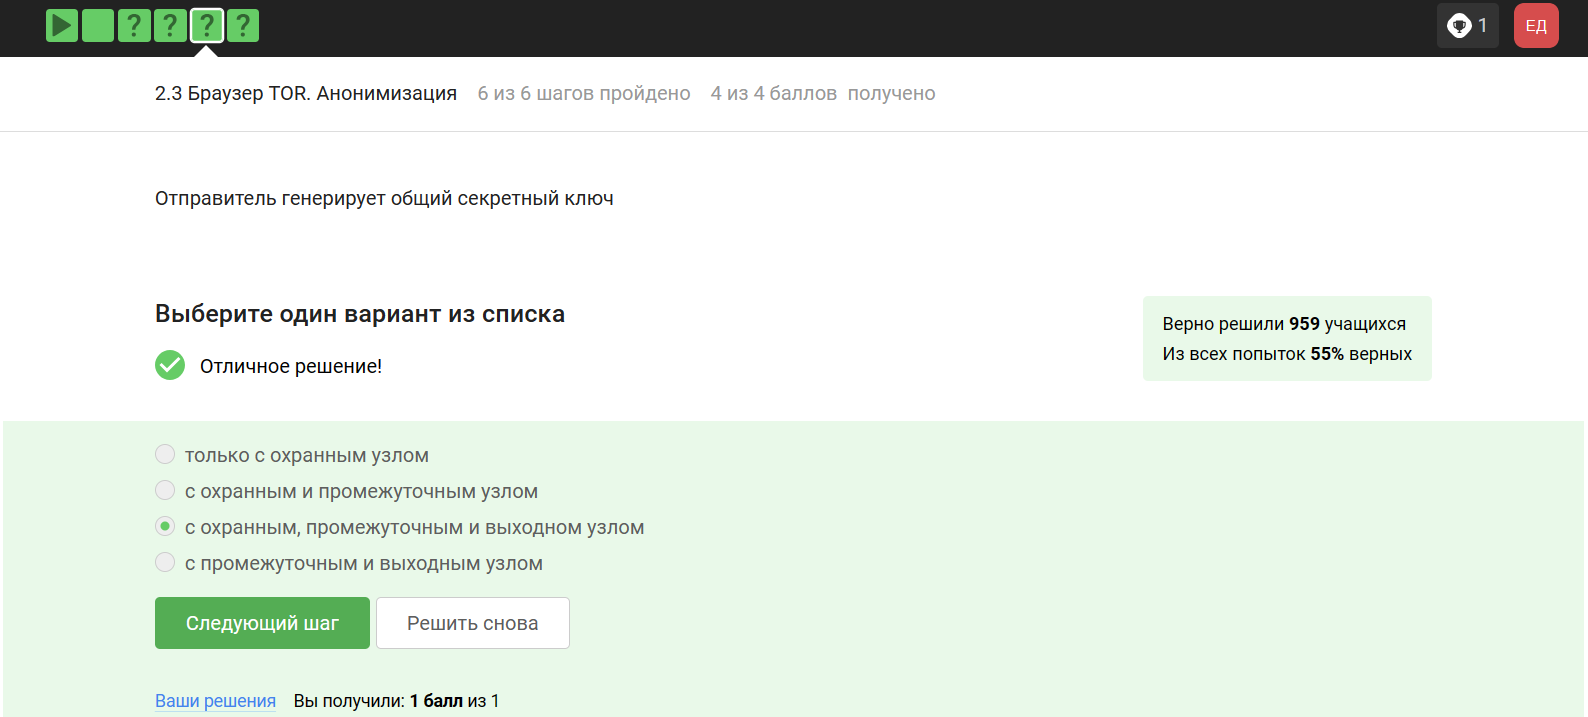
\includegraphics[width=0.7\linewidth,height=\textheight,keepaspectratio]{../report/image/16.PNG}

}

\caption{Вопрос 2.3.3}

\end{figure}%
\end{frame}

\begin{frame}
Для получаения пакетов не нужно использовать TOR. TOR --- это
технология, которая позволяет с некоторым успехом скрыть личность
человека в интернете (рис. {[}-@fig:017{]}).

\begin{figure}

{\centering 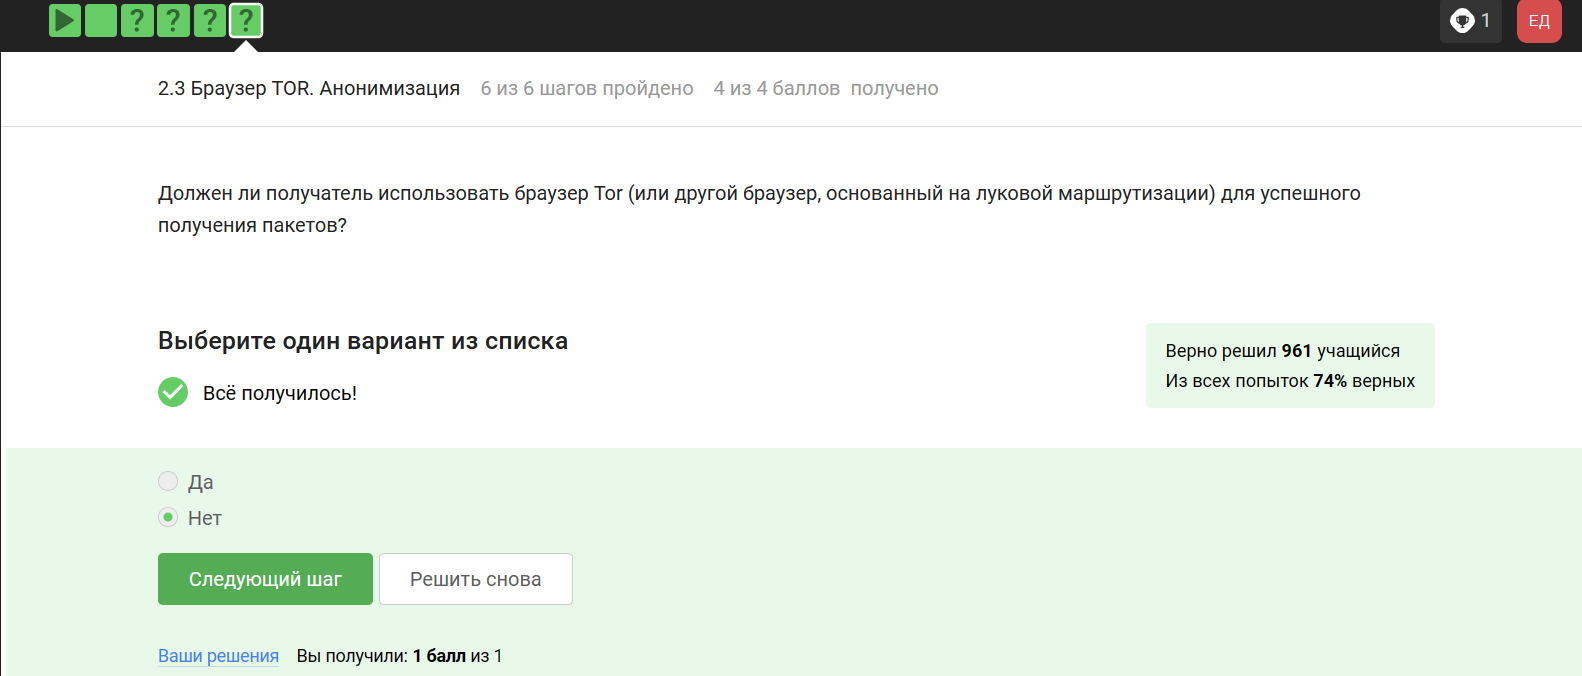
\includegraphics[width=0.7\linewidth,height=\textheight,keepaspectratio]{../report/image/17.PNG}

}

\caption{Вопрос 2.3.4}

\end{figure}%
\end{frame}

\begin{frame}{2.4 Беспроводные сети Wi-fi}
\phantomsection\label{ux431ux435ux441ux43fux440ux43eux432ux43eux434ux43dux44bux435-ux441ux435ux442ux438-wi-fi}
\end{frame}

\begin{frame}
Действительно, это определение Wi-Fi (рис. {[}-@fig:018{]}).

\begin{figure}

{\centering 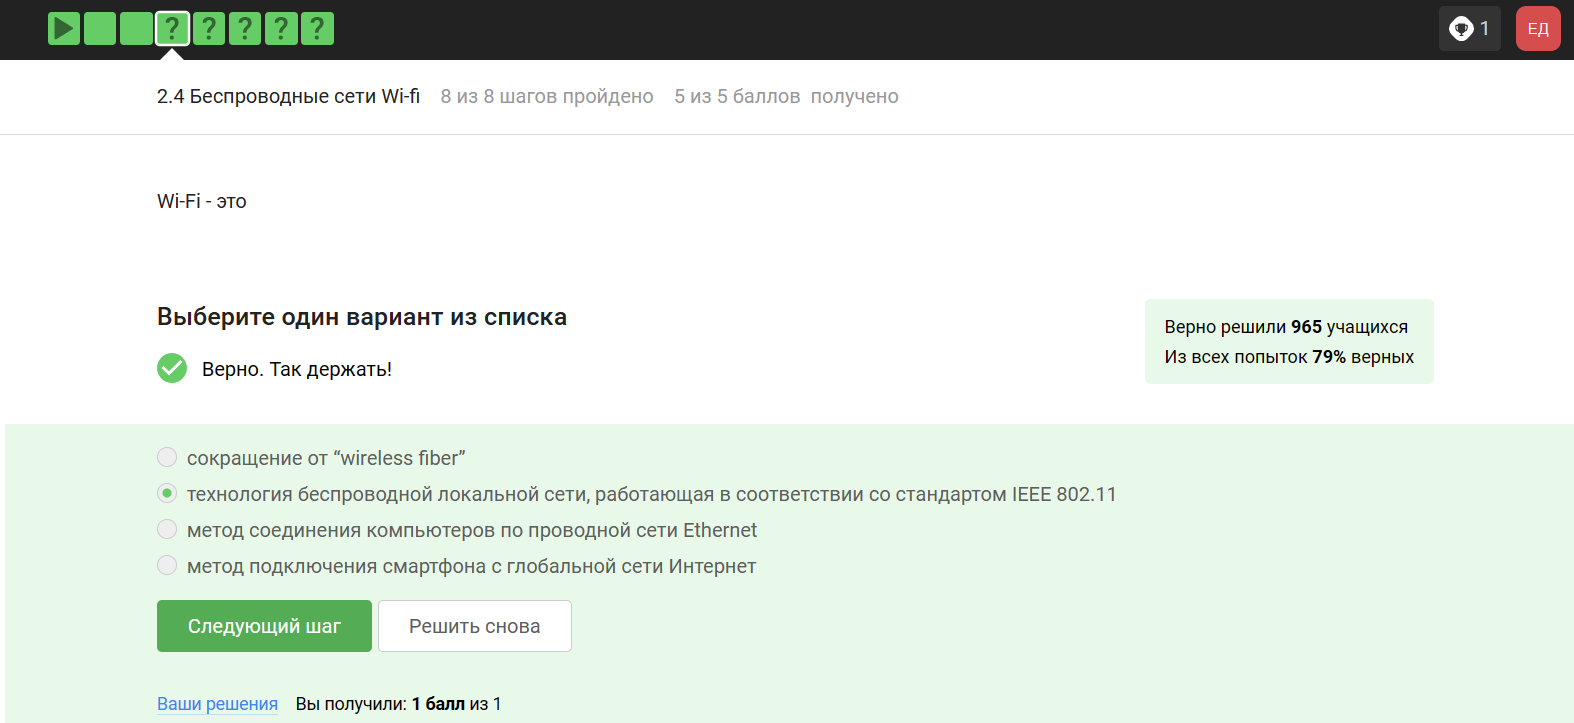
\includegraphics[width=0.7\linewidth,height=\textheight,keepaspectratio]{../report/image/18.PNG}

}

\caption{Вопрос 2.4.1}

\end{figure}%
\end{frame}

\begin{frame}
Для целей работы в Интернете Wi-Fi обычно располагается как канальный
уровень (эквивалентный физическому и канальному уровням модели OSI) ниже
интернет-уровня интернет-протокола. Это означает, что узлы имеют
связанный интернет-адрес, и при подходящем подключении это обеспечивает
полный доступ в Интернет. (рис. {[}-@fig:019{]}).

\begin{figure}

{\centering 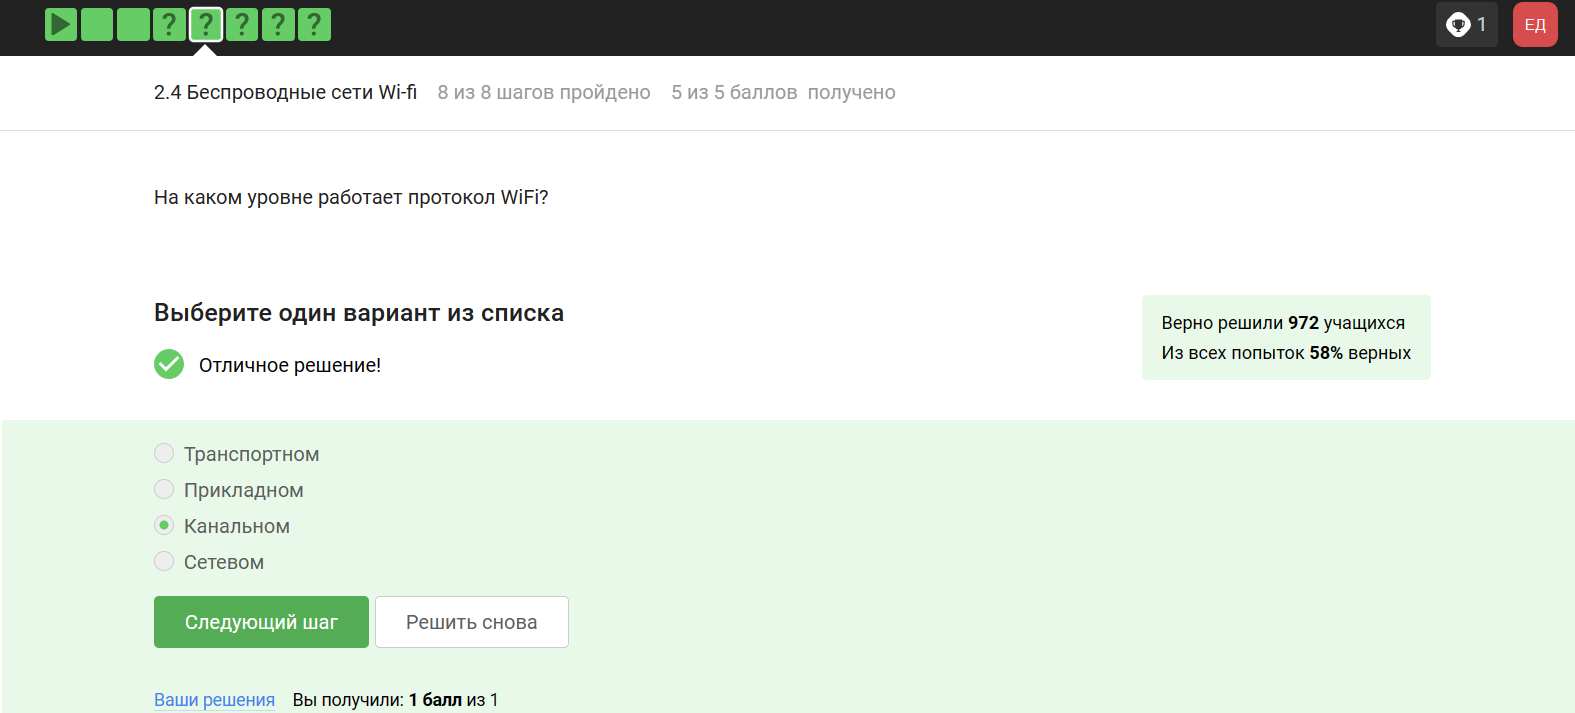
\includegraphics[width=0.7\linewidth,height=\textheight,keepaspectratio]{../report/image/19.PNG}

}

\caption{Вопрос 2.4.2}

\end{figure}%
\end{frame}

\begin{frame}
WEP (Wired Equivalent Privacy) -- устаревший и небезопасный метод
проверки подлинности. Это первый и не очень удачный метод защиты.
Злоумышленники без проблем получают доступ к беспроводным сетям, которые
защищены с помощью WEP, был заменен остальными представленными (рис.
{[}-@fig:020{]}).

\begin{figure}

{\centering 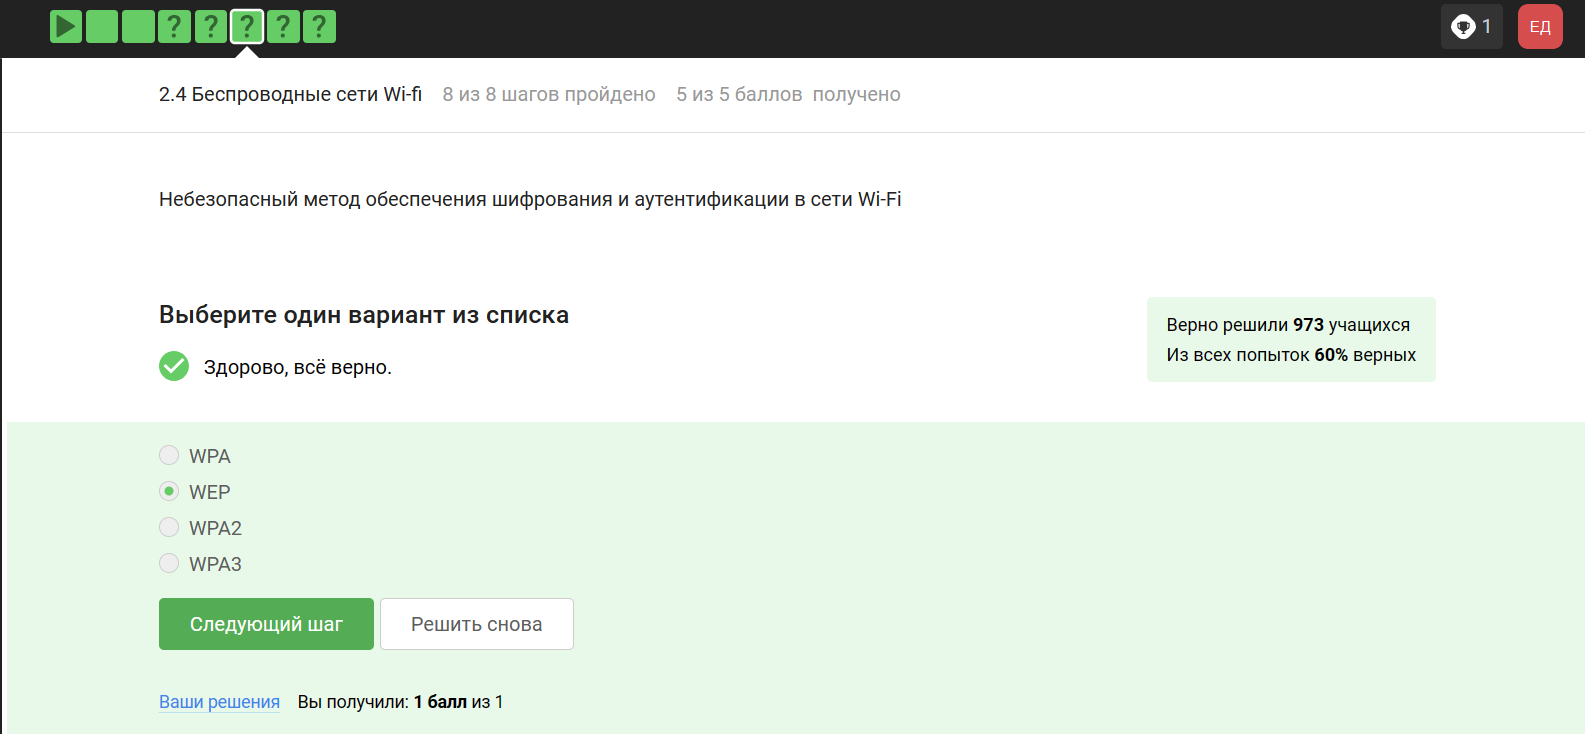
\includegraphics[width=0.7\linewidth,height=\textheight,keepaspectratio]{../report/image/20.PNG}

}

\caption{Вопрос 2.4.3}

\end{figure}%
\end{frame}

\begin{frame}
Нужно аутентифицировать устройства и позже передаются зашифрованные
данные (рис. {[}-@fig:021{]}).

\begin{figure}

{\centering 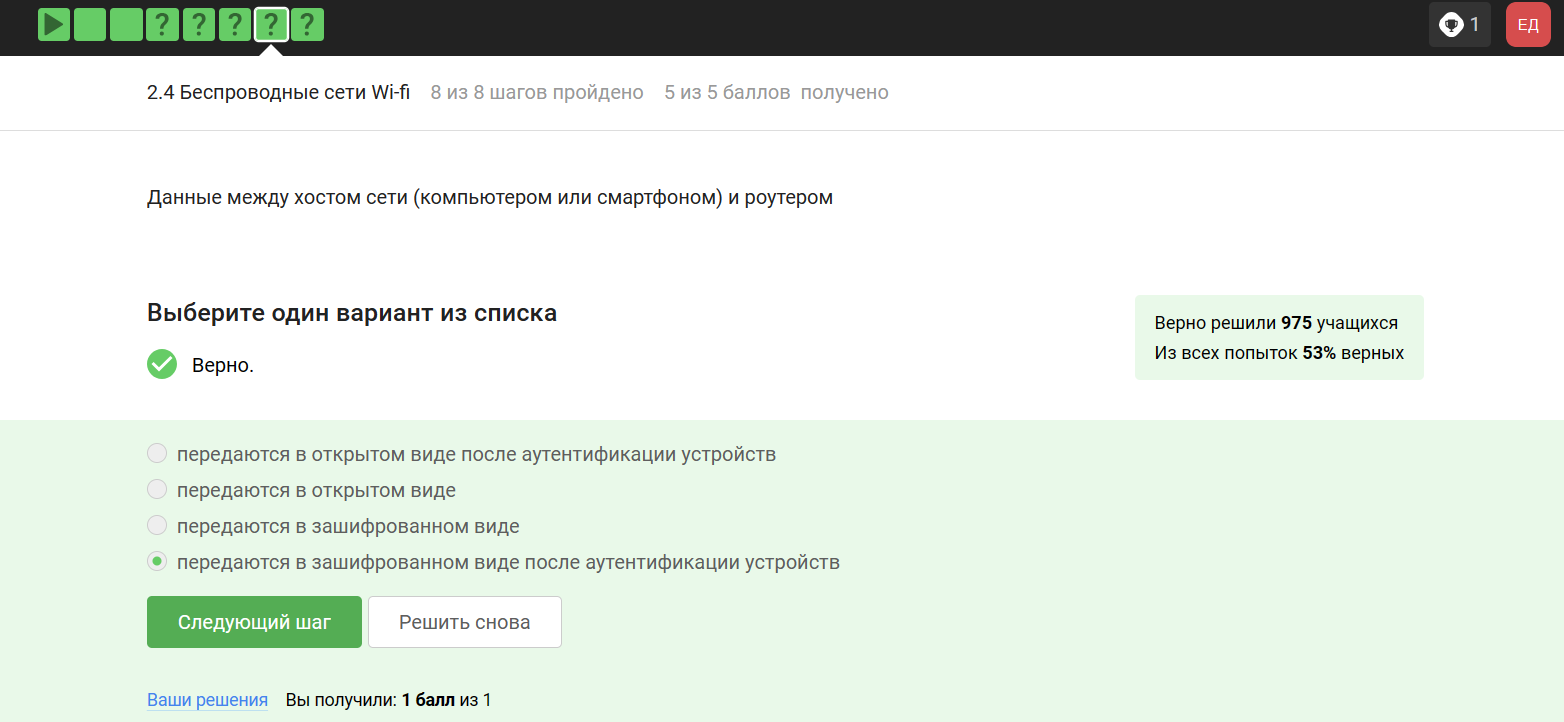
\includegraphics[width=0.7\linewidth,height=\textheight,keepaspectratio]{../report/image/21.PNG}

}

\caption{Вопрос 2.4.4}

\end{figure}%
\end{frame}

\begin{frame}
В целом, понятно по названию, что WPA2 Personal для личного
использования, то есть для домашней сети, enterprise - для предприятий
(рис. {[}-@fig:022{]}).

\begin{figure}

{\centering 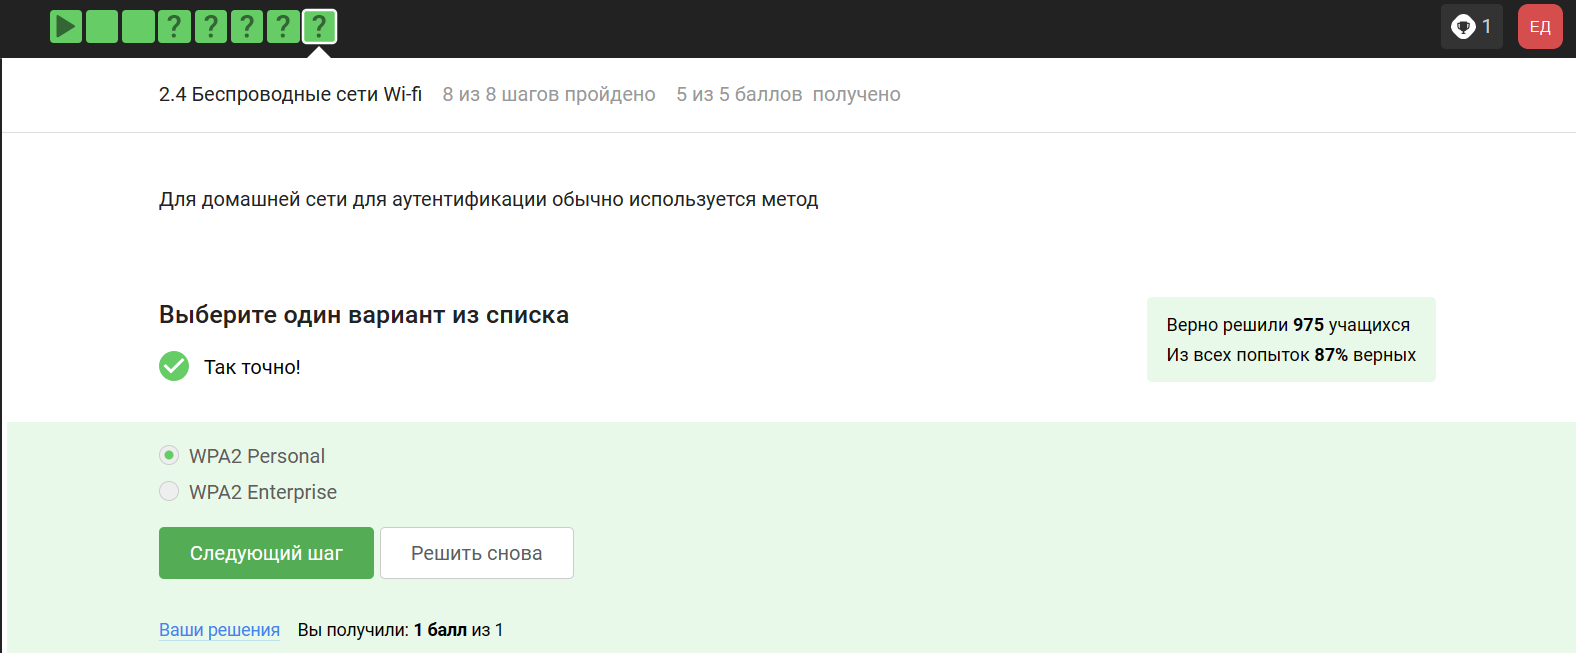
\includegraphics[width=0.7\linewidth,height=\textheight,keepaspectratio]{../report/image/22.PNG}

}

\caption{Вопрос 2.4.5}

\end{figure}%
\end{frame}

\section{3. Выводы}\label{ux432ux44bux432ux43eux434ux44b}

\begin{frame}{3. Выводы}
В ходе выполнения блока \enquote{Безопасность в сети} я узнала о работе
базовых сетевых протоколов, куки сетей Wi-Fi и браузера TOR.
\end{frame}




\end{document}
